\documentclass[12pt, a4paper]{ctexart}

\usepackage{fancyhdr}
\pagestyle{fancy}
\fancyhead{}
\renewcommand{\headrulewidth}{1pt}
\renewcommand{\headwidth}{\textwidth}
\fancyhead[L]{\leftmark}
\fancyhead[R]{\thepage}
\fancyfoot{}

\fancypagestyle{plain}{
\fancyhead{}
\renewcommand{\headrulewidth}{1pt}
\fancyfoot{}
\fancyhead[L]{北京大学基础物理实验报告}
\fancyhead[R]{唐晨宇}
}
\usepackage[colorlinks,linkcolor=red,urlcolor = blue]{hyperref}
\usepackage{booktabs}
\usepackage{graphicx}
\usepackage{amsmath}
\usepackage{mathcomp}
\usepackage{mathabx}
\usepackage{enumitem}
\usepackage[top=1.2in, bottom=1.2in, left=1in, right=1in]{geometry}
\usepackage{tcolorbox}
\usepackage{subfig}

\ctexset{
    section={   
        name={,},
        number={\chinese{section}},
        format=\heiti\raggedright
    },
    subsection={   
        name={(,)},
        number={\chinese{subsection}},
        format=\heiti
    }
}

\begin{document}
\title{迈克耳孙干涉仪\&光源的时间相干性}
\author{唐晨宇 \quad 2300934207}
\date{2024年4月}

\maketitle

\tableofcontents

\clearpage

\section*{实验仪器}

WSM-100迈克耳孙干涉仪,GP200Hg-II低压汞灯,氦-氖激光器,扩束镜(40倍显微镜物镜),橙色玻璃滤光片,黄干涉滤光片,毛玻璃,台灯

\section{迈克耳孙干涉仪调节步骤}

\subsubsection*{步骤一\quad 调节氦-氖激光器水平出射}
将小孔置于靠近氦-氖激光器的位置,调节小孔高度使激光恰好穿过小孔;
再将小孔移至较远处,调节激光器倾角使激光光束再次穿过小孔(“近高远角”)。

\subsubsection*{步骤二\quad 调节激光光束垂直导轨}
调节激光器高度和位置使激光光斑大致处于$M_1$、$M_2$镜中心,保持激光光束通过小孔。
也可以移动迈克尔孙干涉仪来移动光斑位置。

\subsubsection*{步骤三\quad 调节$M'_2$平行$M_1$}
分别调节两个$U_2$螺丝使经过$M_2$反射落在小孔平面上的光斑在横向与纵向上与小孔重合。
然后调节两个$U_1$螺丝使经过$G_1$、$M_1$反射的光斑同时与经过$M_2$反射的光斑和小孔重合(也可先调节$U_1$后调节$U_2$)。

\section{非定域干涉条纹的调节}
\subsection{圆条纹和椭圆条纹的调节步骤}

\begin{description}
    \item[步骤一] 将扩束镜至于光路中,调节扩束镜高度使激光光束经过扩束镜光心。调整扩束镜朝向使经过扩束的光斑中心大致与未扩束时的光斑重合。
    \item[步骤二] 转动M-干涉仪的粗调手轮使光屏上出现较为清晰的条纹,然后调节光屏使干涉条纹大致位于光屏中央。调节两个微动螺丝$U'_2$使$M_1$与$M'_2$平行,从而将圆条纹中心移至光屏中心。
    \item[步骤三] 绕某一位于光屏平面内的轴旋转光屏,即可观察到椭圆条纹。
\end{description}

\subsection{圆条纹的变化规律及解释}

\begin{tcolorbox}
    当$M_1$远离$M'_2$时,圆环中心吐出条纹
    \tcblower
    当$M_1$远离$M'_2$时,两像点源间距增加,中心干涉条纹级次变大。
    由于等倾干涉条纹中心级次大于周围圆环,故原来位于中心的干涉条纹就向周围移动,半径增大,而中心位置则被级次更大的条纹占据,形成“吐条纹”的视觉效果。\\
    反之,当二者靠近时“吞条纹”,原理同上。
\end{tcolorbox}

\begin{tcolorbox}
    当$M_1$远离$M'_2$时,圆环条纹变密
    \tcblower
    两像点源在连线方向干涉公式$2d \cos \theta_k = k \lambda \Rightarrow \Delta \theta_k = \frac{\lambda}{2d \sin \theta_k}$\\
    当$M_1$远离$M'_2$时,两像点源间距$d$增大,由上述公式得$\Delta \theta_k$减小,故干涉条纹宽度$f \Delta \theta_k$减小即条纹变细密。
    从另一个角度出发,视场范围一定即视场边缘的角度$\theta_m$一定,而$k \lambda$的变化范围为$2d (1 - \cos \theta_m),\theta_m \ll 1$。
    当$d$增大时,$k \lambda$的变化范围增大,视场中的干涉条纹级数增多,干涉条纹自然应该变密。
\end{tcolorbox}

\begin{tcolorbox}
    $d$与$r_k$的关系
    \tcblower
    从上述推导中我们可以得出,$2d \frac{\theta_k^2}{2} = (k_0 - k)\lambda \Rightarrow r_k \approx f \theta_k = f \sqrt{\frac{(k_0 - k) \lambda}{d}}$\\
    代入$d = k_0 \lambda$,我们得到$r_k = f \sqrt{2 - \frac{k \lambda}{d}}$,其中$f$为两像电源至光屏的距离,$k_0$为干涉圆心处条纹级次。
\end{tcolorbox}

\section{非定域直条纹和双曲条纹的调节方法}
调节两个微动螺丝$U'_2$使经过$M_2$反射的像点偏离$M_1$像点所在轴线。
然后转动M-干涉仪的粗调手轮,此时会看到双曲条纹。
继续转动手轮直至两像点源连线平行光屏所在平面,此时我们可以看到较为清晰的直条纹。

反复调节$U'_2$即可改变条纹间距。

\section{定域干涉等倾条纹的调节方法}

\paragraph{调节方法}
重复二(一)中步骤使非定域圆条纹圆心位于视场中央并调节至条纹粗而疏的状态($d$小)。
撤去光屏,在扩束镜与$G_1$间插入毛玻璃片形成扩展光源。
此时用眼睛聚焦无穷远,我们可以看到定域的等倾干涉圆条纹。
调节两个微动螺丝$U'_2$,分别对应左右倾角和上下倾角。
使眼睛上下左右移动,分别调节相应的微调螺丝。
当眼睛移动时条纹不再吞吐,此时就是严格的等倾条纹。

\paragraph{原理说明}
当眼睛移动时观察到条纹吞吐,表明不同位置的0级(垂直)出射光仍有光程差,即$M_1$和$M'_2$仍未严格平行。

\section{等倾条纹的变化规律及解释}
等倾干涉中严格有$2d \cos \theta_k = k \lambda$,形式上与两点源完全相同,故各项特征、变化规律及解释与三中描述均一致,此处不再重复。

\section{定域干涉等厚条纹的调节方法}
调节两个微动螺丝$U'_2$使$M'_2$镜与$M_1$镜夹一小角,此时干涉圆心会移出视场。
用眼睛聚焦在$M_1$附近即可观察到等厚干涉条纹。
转动M-干涉仪的粗调手轮使干涉条纹向远离圆心的方向移动,再次反复调节两个微动螺丝$U'_2$使条纹间距较大而保持清晰,直至视场中条纹基本平行即可。

\section{等厚条纹的变化规律及解释}
旋转粗调手轮,可以看到条纹向一个方向移动,由向一边弯曲变成直条纹,紧接着又变成向另一边弯曲,这就是定域干涉等厚条纹的基本特征。
等厚干涉近似满足$2d \cos \theta = k \lambda$,其中$d = d_0 + x \alpha$,$\alpha$为$M_1$和$M'_2$夹角且$\alpha \ll 1$。
近似有$\theta \ll 1$,故$\Delta L = 2d (1 - \frac{\theta^2}{2})$。
在$M_1$和$M'_2$交棱附近$\frac{\theta^2}{2}$项可忽略,但当$d$逐渐变大时$d\theta^2$项不可忽略,条纹出现弯曲现象。

由上述公式可算得条纹间距$\Delta x = \frac{\lambda}{2\alpha}$,可见当$M_1$和$M'_2$夹角变大时条纹间距减小。

\section{白光等厚干涉条纹的调节方法及干涉条纹的现象描述}

氦-氖激光的相干长度非常长,所以我们可以在非常宽的范围内看到干涉条纹。
但是白光的频谱并不像激光那样是个非常尖锐的峰,这导致白光干涉条纹仅在光程差为0的附近才能看到,光程差变大后条纹可视度迅速下降,条纹变得模糊不可见。
因此,本实验先需要把$M_1$与$M'_2$的交棱调到视场正中,然后在已经看见交棱附近平行度较好的激光干涉条纹后打开台灯作为白光光源,
适当调节粗调和细调手轮、$M_2$的倾角即可观察到0级白色条纹(可能是0级暗纹)和两侧的彩色条纹。

\section{观测不同光源的相干长度}

\paragraph{白光} 仅用白光进行干涉,如图\ref{fig 2-1},我们可以看到的完整干涉条纹只有0级和$\pm 1$级三条暗纹,故取白光平均波长$\lambda_1 = 550 nm$,$k_1 = 1$,
则相干长度$\Delta L_{1max} = k_1 \lambda_1 = 550nm $,相干时间$t_1 = \frac{\Delta L_{1max}}{c} = 1.83 fs$。

\paragraph{白光经橙色玻璃滤光} 在白光光源后加入一块橙色玻璃进行滤光,如图\ref{fig 2-2},缩减频谱宽度后再次观测干涉条纹,可以得到$k_2 = 19$。
取波长$\lambda_2 = 625 nm$,算得$\Delta L_{2max} = k_2 \lambda_2 = 11.875 \mu m$,相干时间$t_2 = \frac{\Delta L_{2max}}{c} = 39.6 fs$。

\paragraph{白光经黄干涉滤光片滤光} 在白光光源后加入黄干涉滤光片,如图\ref{fig 2-3},观测得到$k_3 = 64$。
取波长$\lambda_3 = 578 nm $,算得$\Delta L_{3max} = k_3 \lambda_3 = 36.992 \mu m$,相干时间$t_3 = \frac{\Delta L_{3max}}{c} = 123.4 fs$。

\paragraph{低压汞灯黄光} 在低压汞灯后加入黄干涉滤光片,测量得到等光程位置$d_0 = 51.379mm$;
转动粗调手轮至第一次完全看不清干涉条纹(注意不是波节,以圆环中心消失为标准),测得在$d_{max} = 68.000mm$附近条纹完全消失,
故$\Delta L_{4max} = 2(d_{max} - d_0) = 33.242mm$,相干时间$t_4 = \frac{\Delta L_{4max}}{c} = 110.88 ps$。

\begin{figure}[htbp]
    \centering
    \subfloat[白光]{
        \label{fig 2-1}
        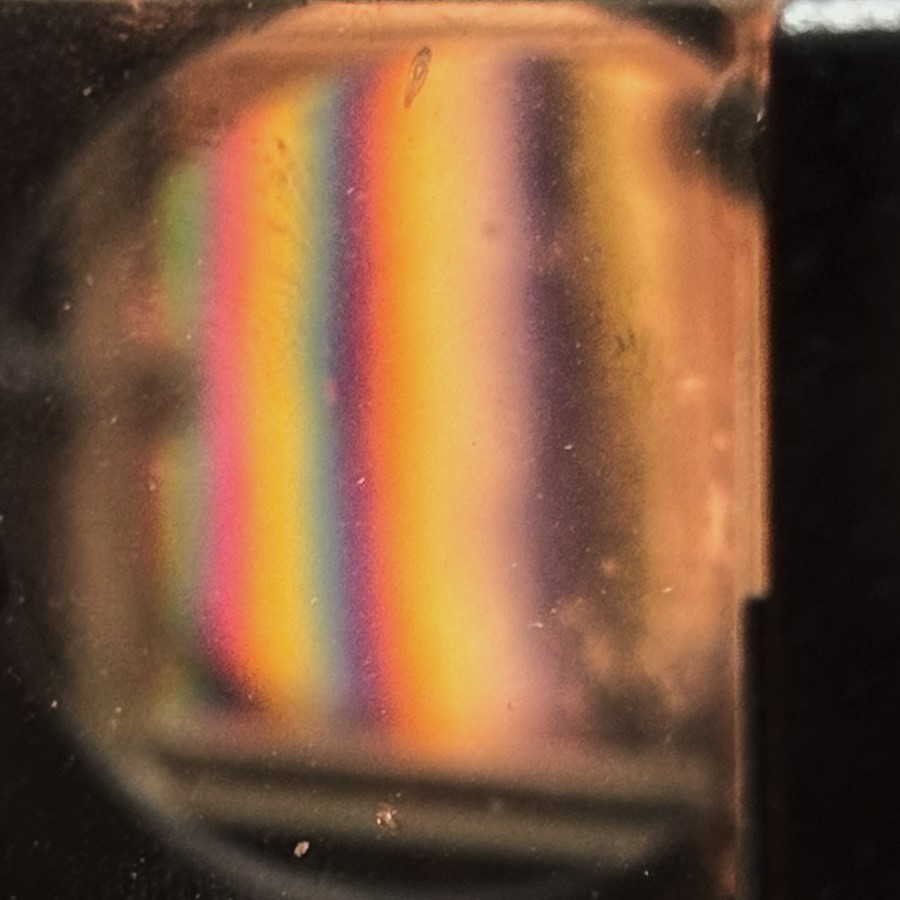
\includegraphics[width = 2in]{白光.jpg}
        }
    \subfloat[橙色玻璃滤光]{
        \label{fig 2-2}
        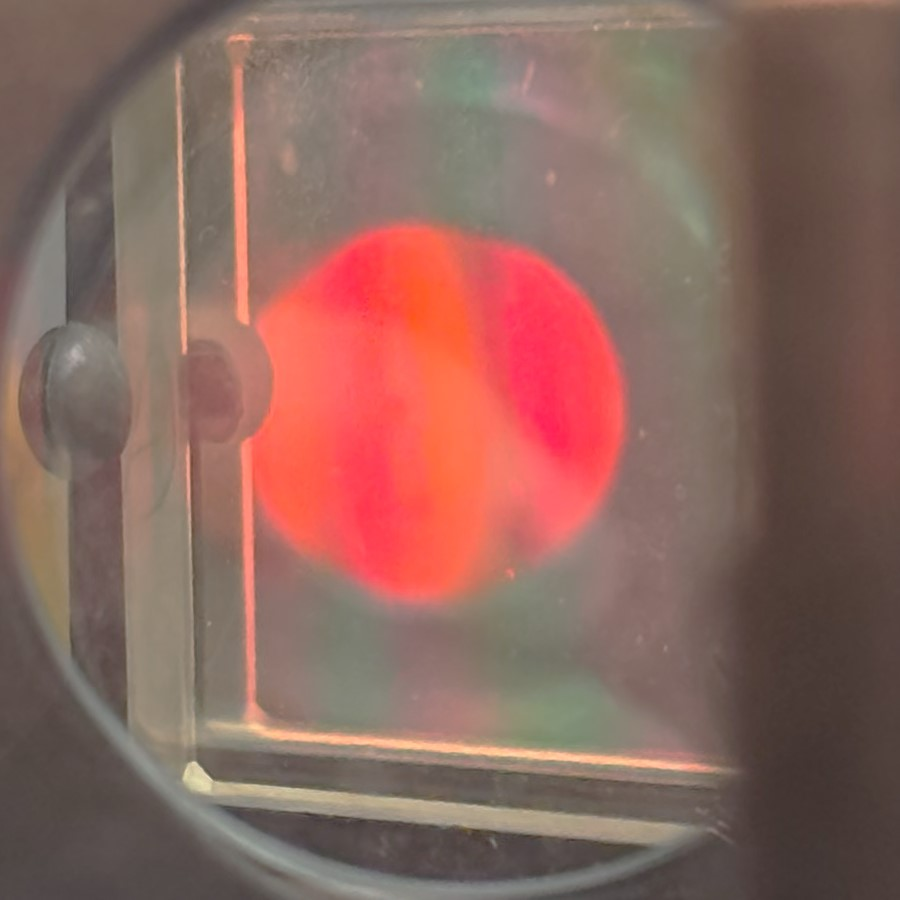
\includegraphics[width = 2in]{橙色滤光.jpg}
        }
    \subfloat[黄干涉滤光片滤光]{
        \label{fig 2-3}
        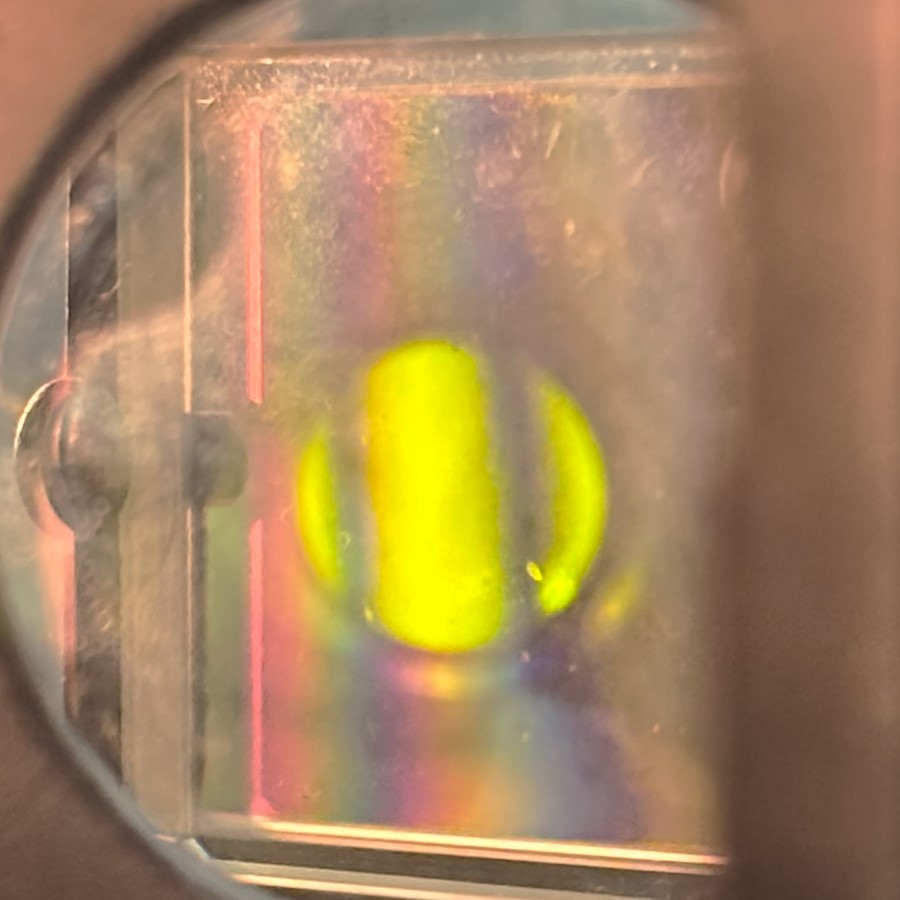
\includegraphics[width = 2in]{黄干涉滤光.jpg}
        }
    \caption{不同光源的干涉条纹}
\end{figure}

\section{测定汞黄光双线的波长差}
\subsection{测量衬比度拍频}

部分衬比度变化波节坐标如下:

\begin{table}[htbp]
  \centering
  \caption{衬比度波节坐标}
    \begin{tabular}{cccccc}
    \toprule
    $i$     & 1     & 3     & 4     & 5     & 6  \\
    \hline
    $d_{i}/mm$ & 49.93664 & 50.09529 & 50.17600 & 50.25595 & 50.33496 \\
    \midrule
    $i$     & 7     & 8     & 10    & 13    & 14 \\
    \hline
    $d_{i}/mm$ & 50.41395 & 50.49527 & 50.65645 & 50.89157 & 50.96922 \\
    \bottomrule
    \end{tabular}
  \label{tab:t1}
\end{table}

\begin{figure}
    \centering
    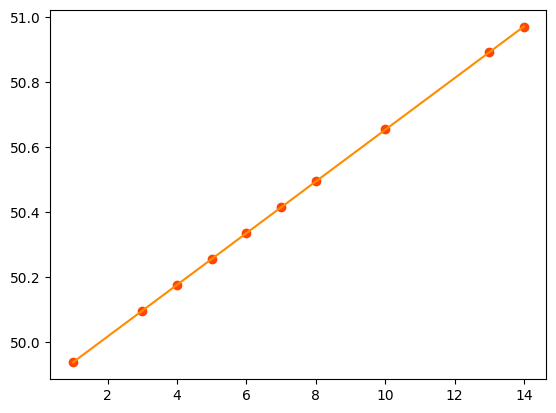
\includegraphics[width = 3in]{波节拟合.png}
    \caption{衬比度拍频拟合线}
\end{figure}

最小二乘法拟合得$\Delta d = 0.07955 mm$,$r = 0.999990$\\
有\[ \frac{\sigma_{A \Delta d}}{\Delta d} = \sqrt{\frac{1/r^2 - 1}{n - 2}} \Rightarrow \sigma_{A \Delta d} = 0.00013mm \]

取估测得到的人眼无法分辨范围为极限系统误差$e = 0.0001mm$,\\
算得\[ \sigma_{\Delta d} = \sqrt{\sigma_{A \Delta d}^2 + \frac{e^2}{3}} = 0.00015 mm \]
故取平均波长$\bar{\lambda} = 578.0nm$,最终结果为$\Delta \lambda = \frac{\bar{\lambda}^2}{2 \Delta d} = 2.100nm$,
不确定度$\sigma_{\Delta \lambda} = \frac{\partial \Delta \lambda}{\partial \Delta d} \sigma_{\Delta d} = 0.004mm$。

\subsection{测量相邻波腹间的干涉条纹数目}

从用光电自动记录画出的汞黄双线干涉图(见图\ref{fig 2})中,我们数出两相邻波节间条纹数目为$\Delta k = 272$,
代入公式得$\Delta lambda = \frac{\bar{\lambda}}{\Delta k} = 2.125nm$,与上一种方法得到结果之间的误差基本在接受范围内。

\begin{figure}
    \centering
    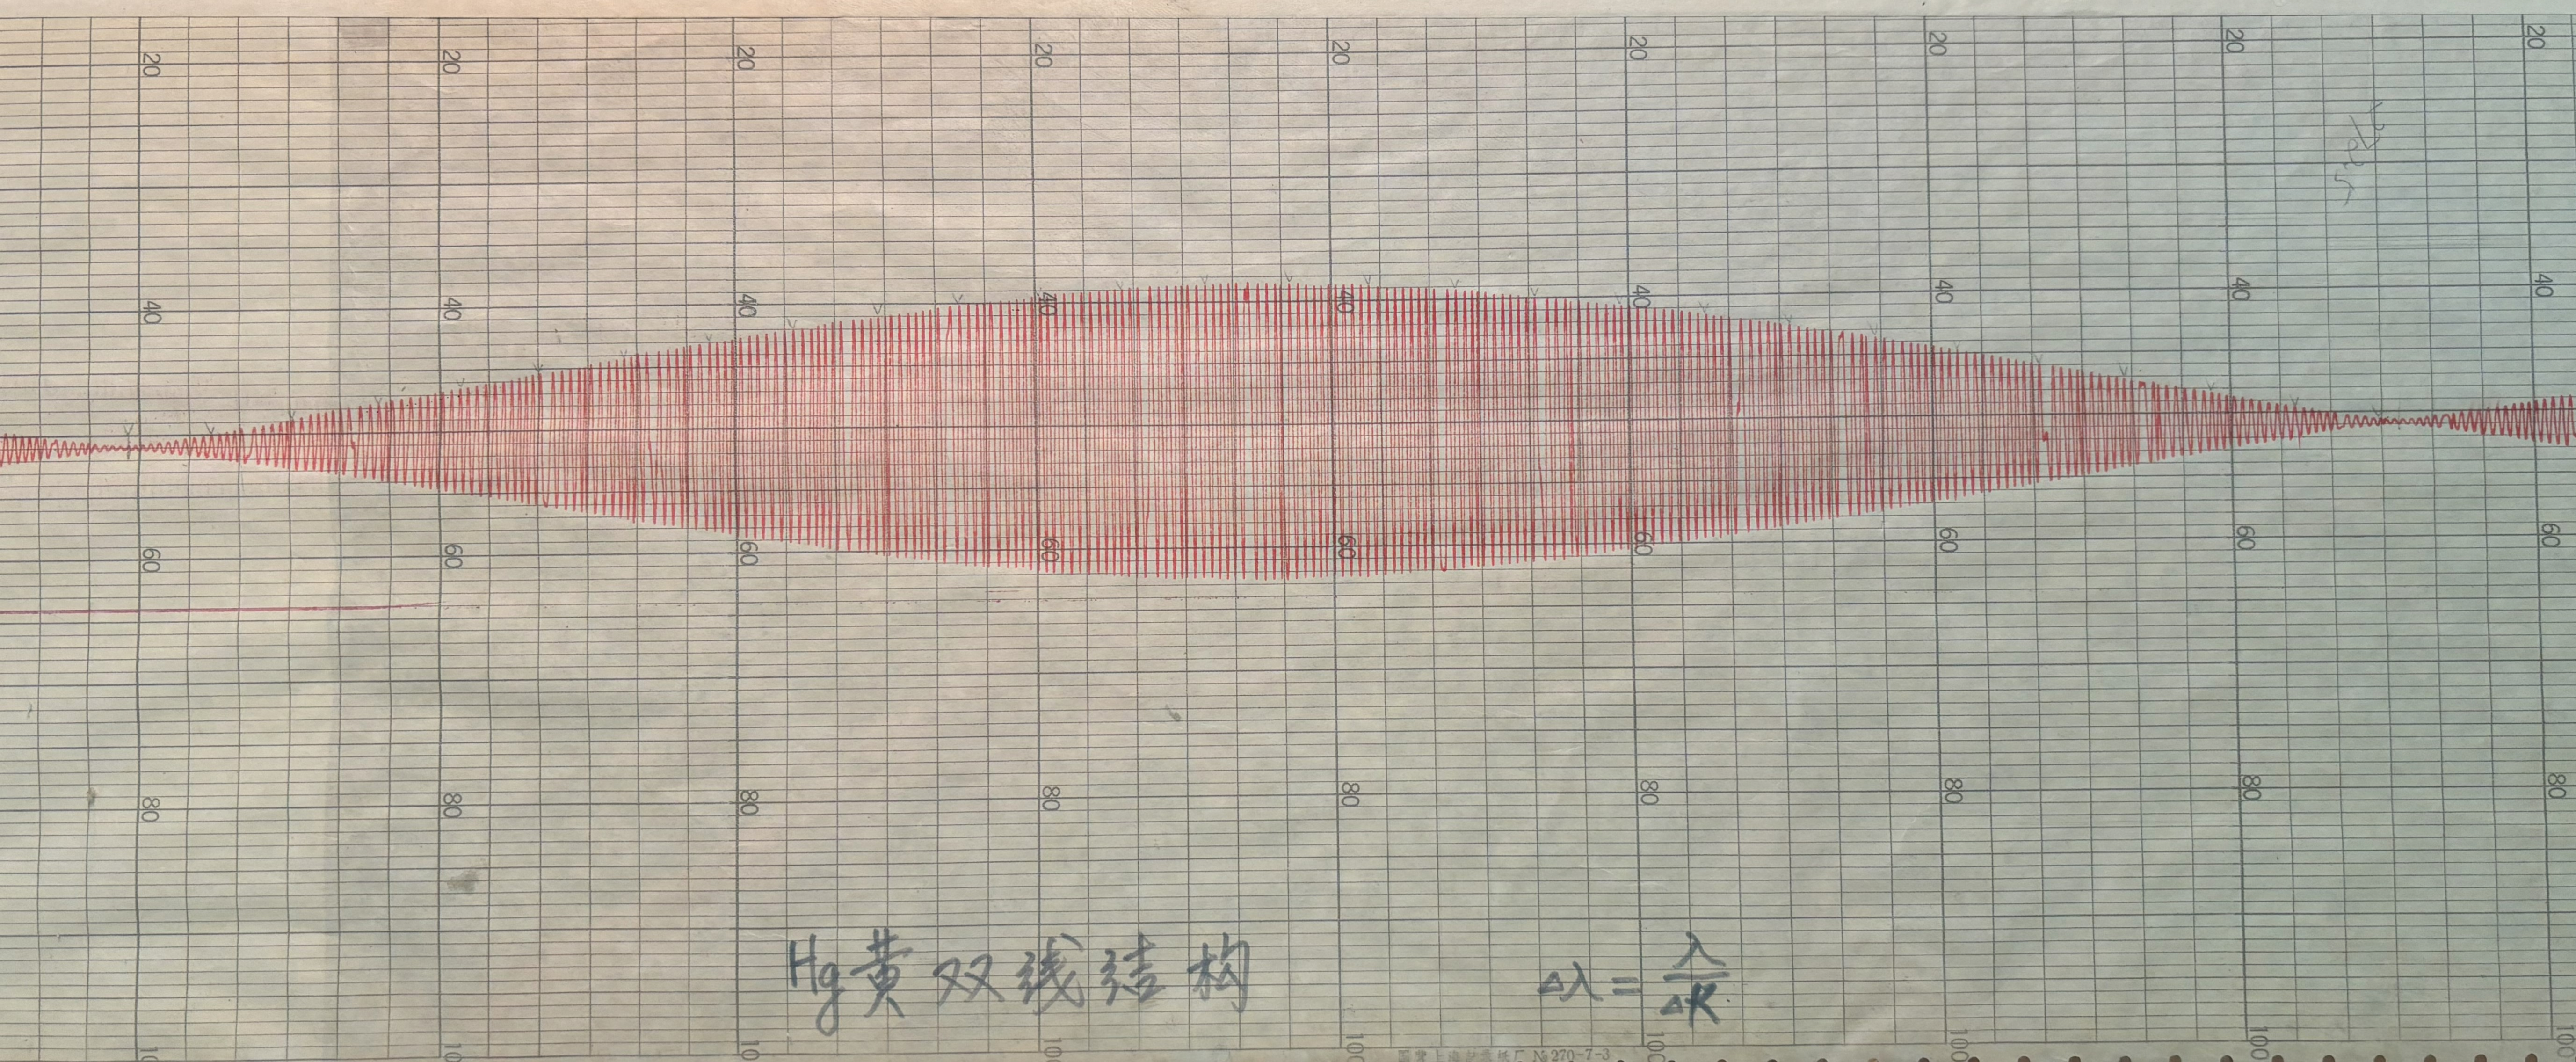
\includegraphics[width = 5in]{光电转换结果.jpg}
    \caption{干涉条纹光电转换图像}
    \label{fig 2}
\end{figure}


\end{document}
